\documentclass[conference]{IEEEtran}
% The preceding line is only needed to identify funding in the first footnote. If that is unneeded, please comment it out.
\usepackage{cite}
\usepackage{amsmath,amssymb,amsfonts}
\usepackage{algorithmic}
\usepackage{graphicx}
\usepackage{textcomp}
\usepackage{xcolor}
\def\BibTeX{{\rm B\kern-.05em{\sc i\kern-.025em b}\kern-.08em
    T\kern-.1667em\lower.7ex\hbox{E}\kern-.125emX}}
\begin{document}

\title{Classifying Speakers in Audio Recordings using MedleyVox Dataset
}

\author{\IEEEauthorblockN{Rahul Jain}
\IEEEauthorblockA{\textit{Department of Computer Science} \\
\textit{Pomona College}\\
Claremont, CA \\
rjaa2020@mymail.pomona.edu}
\and
\IEEEauthorblockN{Nannapas Wonghirundacha}
\IEEEauthorblockA{\textit{Department of Computer Science} \\
\textit{Pomona College}\\
Claremont, CA \\
nwab2020@mymail.pomona.edu}
}
\maketitle

\begin{abstract}
In our project, we present a novel method for identifying the number of distinct singing voices in audio tracks using the MedleyVox dataset. 
Our approach for this task involves a three-tiered strategy. Initially, we focused on employing high-dimensional embeddings and clustering algorithms to identify unique vocal clusters. Progressing further, we explored the use of Pyannote, an advanced speech diarization toolkit, for more nuanced voice separation. The culmination of our efforts was the development of a Recurrent Neural Network (RNN) model, particularly leveraging Long Short-Term Memory (LSTM) networks, to process sequential audio data. This model was adept at recognizing individual vocal signatures and distinguishing between singers by analyzing their unique timbre and style.

The innovative aspect of our approach was in how the LSTM model processed the audio embeddings and detected shifts in vocal characteristics, marked as 'switches'. The final model demonstrated a significant improvement in accuracy, showcasing our project's contribution to the field of automated vocal analysis. This research not only enhanced our understanding of machine learning and audio analysis but also opens up new possibilities for advanced audio separation models in various sectors, especially entertainment and assistive technologies.
\end{abstract}

\begin{IEEEkeywords}
Signal Processing, Music Recognition, Audio Embedding, LSTM, RNN, SpeechBrain, PyTorch
\end{IEEEkeywords}

\section{Introduction}
MedleyVox is a cutting-edge evaluation dataset, developed to address the intricate challenge of separating multiple singing voices in audio tracks. This dataset is unique in its comprehensive scope, covering various complex scenarios like duets, unison, main versus rest, and N-singing separations [1]. It provides a rich resource for researchers and developers, furnishing them with a diverse range of audio samples that represent real-world challenges in music source separation. A fundamental question that drives our research with this dataset is: given an audio recording, can we classify how many singers are singing?

MedleyVox's detailed and varied dataset is crucial for advancing audio processing algorithms, particularly for isolating individual voices in music production and audio engineering. Utilizing the MedleyVox `duet' dataset, our project aims to create a model that identifies the number of distinct voices in a song, challenging our understanding of machine learning and the limits of existing models. This endeavor encompasses three levels of complexity:

\begin{enumerate}
    \item \textbf{Clustering:} Initially, we adopted a simpler method, using minimal preprocessing and analysis techniques. In this phase, songs were represented as high-dimensional embeddings, and a clustering algorithm was tasked with determining the number of distinct clusters, each potentially representing a unique voice.
    \item \textbf{Pyannote Speaker Diarization:} In the second phase, we explored Pyannote, a speaker diarization toolkit, to refine our voice separation capabilities. Pyannote's advanced algorithms provided a more nuanced approach to identifying distinct vocal tracks within the complex audio data.
    \item \textbf{Supervised Learning an RNN:} Our final strategy involved constructing a model from scratch using Pytorch, drawing on the semester's learnings. We opted for Recurrent Neural Networks (RNNs) owing to the sequential nature of audio data. This approach aimed to capitalize on the distinct temporal characteristics of each singer's voice within a track.
    \end{enumerate}

By sidestepping a classification system that identifies each singer individually, our project not only aims to discern unique vocal signatures in songs but also to detect shifts in these signatures. This challenge is akin to 'zero-shot learning' in machine learning, where the model must generalize to new, unseen instances, thereby pushing the boundaries of conventional audio processing techniques.

Through this project, we are not only enhancing our understanding of audio analysis and machine learning but also contributing to the broader field by tackling a problem that simulates real-world scenarios in voice recognition and separation. The project's outcomes could pave the way for more sophisticated models in the future, capable of handling increasingly complex audio separation tasks, an advancement with far-reaching implications in various sectors from entertainment to assistive technologies.

\section{System Design}
\subsection*{Preparing our Dataset and Pre-processing}

We utilized the existing MedleyVox dataset containing isolated vocal tracks from over 100 songs performed by a diverse group of singers. Specifically, this dataset includes 21 duet songs with vocals from a total of 42 unique singers.

To construct our new dataset, we harnessed these 21 pre-existing duets and their associated isolated vocals. By randomly combining the solo vocal clips of different singers from this pool, we created new arrangements made up of 2-7 unique singers.

\begin{figure}[ht]
    \centering
    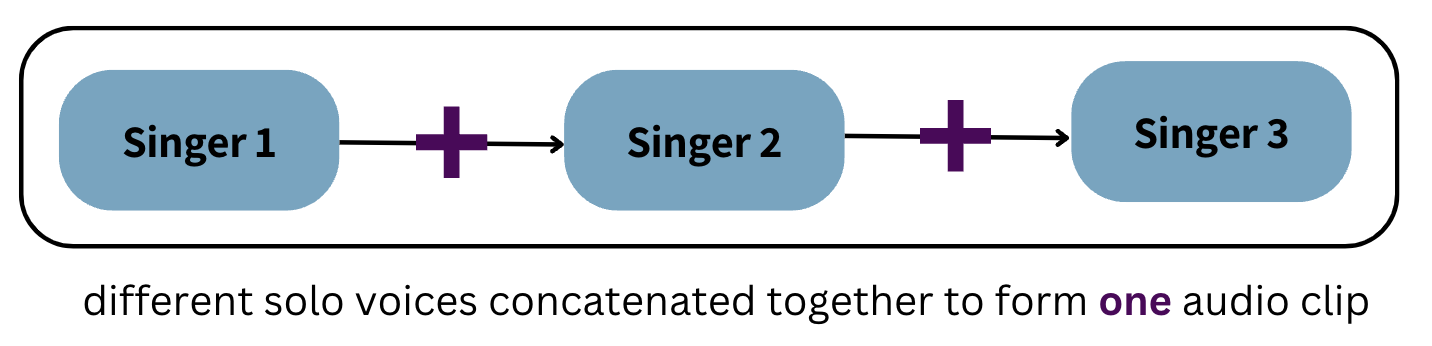
\includegraphics[scale=0.25]{Singer.png}
    \caption{A diagram of how we generated our dataset.}
    \label{fig:Data}
\end{figure}

\subsubsection{Split Audio into Chunks}
First, we divided the full audio recording into equal chunks for analysis. Breaking the long recording into shorter segments allowed for comparison of smaller sections.

\subsubsection{Generate Embeddings}
Next, we input each chunk into a pre-trained SpeechBrain Encoder Classifier model to generate embeddings. This state-of-the-art model for speaker recognition was trained on a diverse speech dataset (VoxCeleb) to effectively represent key vocal features including accent, age, gender etc [3][4]. Using this model we output embeddings for each chunk.

\begin{figure}[ht]
    \centering
    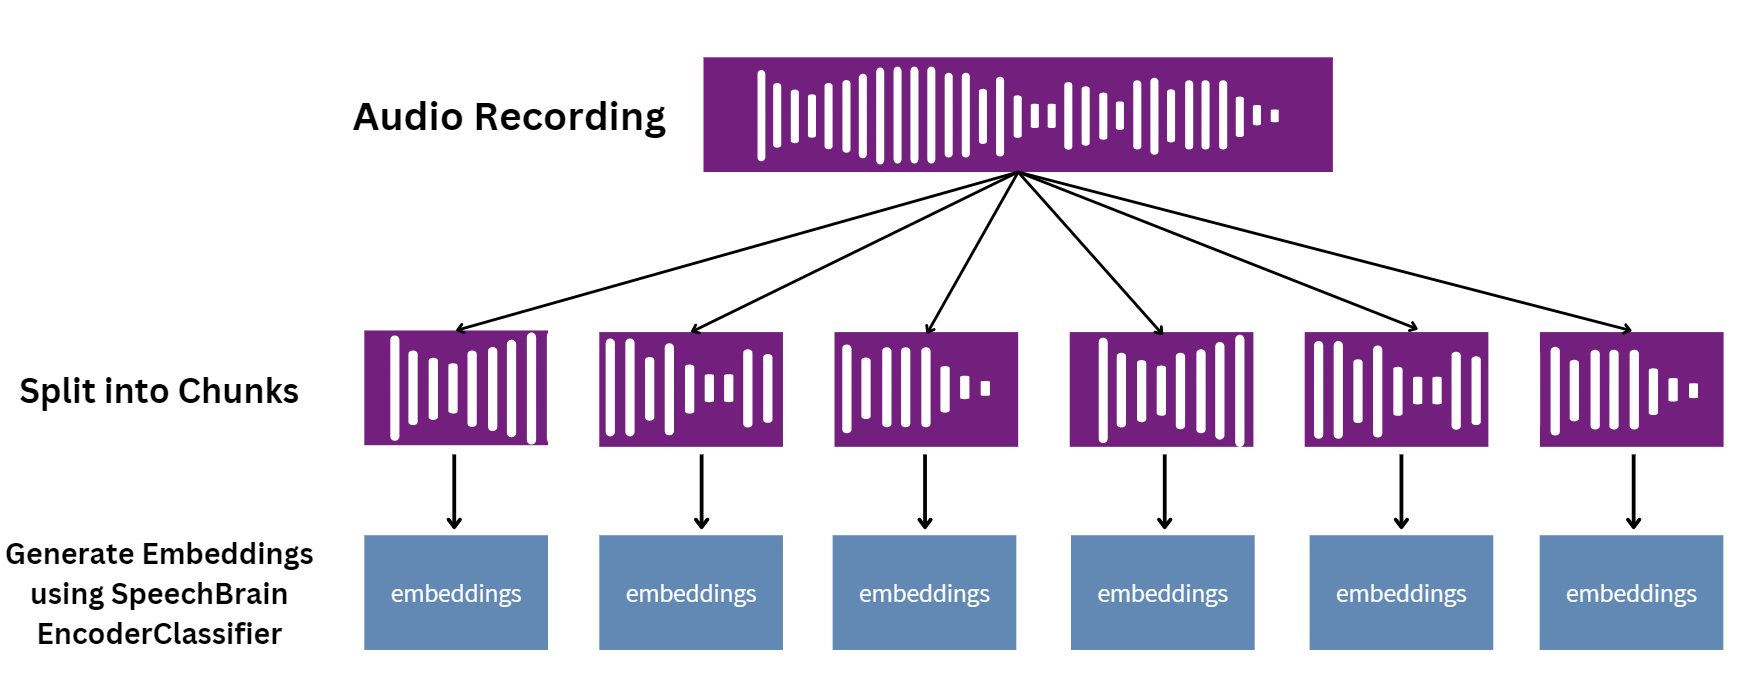
\includegraphics[scale=0.25]{chunking.png}
    \caption{A diagram of how we preprocessed our generated ``songs" for this task. Starting with an audio clip of $n$ singers, we evenly split the audio into $c$ chunks of audio. These $c$ chunks were then passed through the \textit{EncoderClassifier} from the \textit{SpeechBrain} library.}
    \label{fig:chunking}
\end{figure}

\begin{figure}[ht]
    \centering
    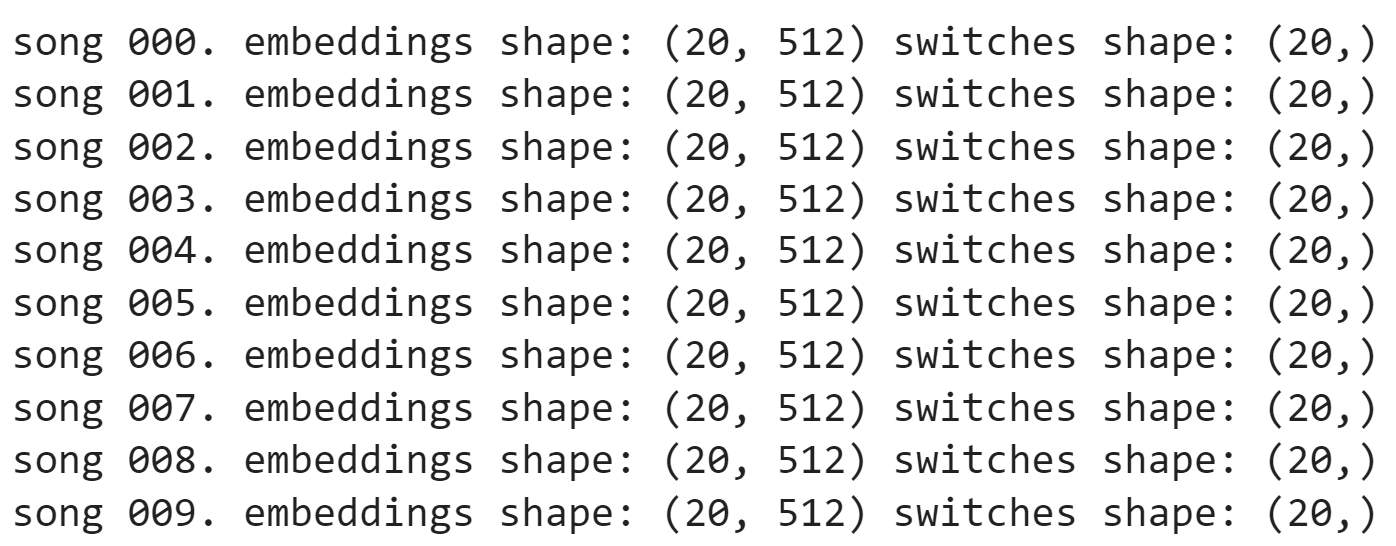
\includegraphics[scale=0.25]{enbeddings_and_switches.png}
    \caption{After splitting each song into $n$ embedded chunks, each ``song" was represented as a $n$ x 512 tensor}
    \label{fig:embeddings}
\end{figure}

As this multi-singer detection task is novel and lacks established benchmarks, we implemented two state-of-the-art models (Approach A and B) to evaluate against our proposed RNN approach.

\subsection{Approach A: Clustering}
\subsubsection{Perform Dimensionality Reduction}
The initial embeddings output by the SpeechBrain Encoder Classifier contained many features to represent the audio characteristics. However, working with such high dimensional representations can be unwieldy. Therefore, we applied Principal Component Analysis (PCA), a common technique for dimensionality reduction, to simplify the embeddings. PCA identifies the key components that account for the majority of the variance in high-dimensional data. Specifically, we set the target dimension of the PCA output based on the expected number of singers. For example, when working with a dataset with only 2 singers, we would reduce down to 1-2 component dimensions. If there were 5 singers, may reduce to 3-4 components. Condensing the data this way eliminates noise while preserving the most meaningful latent traits. In simple terms, whereas our audio chunks were originally described by many numerical features from the neural network embeddings, they are now represented by just 1, 2 or 3 values that encapsulate the core elements determining differences between the chunks.

\subsubsection{Mean-Shift Clustering}
To group similar chunks and thus identify distinct singers, we leveraged a Mean-Shift clustering algorithm. Mean-Shift is an unsupervised machine learning technique, meaning it finds patterns in the data without predefined labels or categories.  We selected Mean-Shift because it automatically detects the number of clusters emerging from the similarities in the data itself - ideal for clustering based solely on the chunk embeddings without singer identity labels provided for supervision.

\subsection{Approach B: Pyannote Speaker Diarization}
Our second methodology employs the pre-trained Pyannote Speaker Diarization 3.0 model for raw audio input without data pre-processing requirements. This model is originally trained on diverse datasets primarily consisting of speaker data and excels in detecting different speakers in an audio stream. It outputs speaker timestamps in the form of Rich Transcription Time Marked (RTTM) files [2]. By feeding the multi-singer recordings directly into Pyannote, we obtained predicted speaker turn patterns within the long recordings over time. Parsing the timestamps allowed classification of number of detected vocalists. 

\subsection{Approach C: Sequential Chunk Processing with RNN}

Building off our previous approaches, we decided to implement a model of our own to count the number of singers in an audio recording. We chose to use a Recurrent Neural Network (RNN), which processes data sequentially. Specifically, we used a Long Short-Term Memory (LSTM) Layer, which emulates human memory by keeping track of both short-term changes and long-term dependencies within the data. In this context, the model would learn the sound of a specific singer by comparing the audio embeddings at chunk $n$ to embeddings from previous chunks.

\subsubsection{Preparing our data for the model}
Our model took the pre-processed SpeechBrain embeddings for each audio chunk as input (Figure 2). The corresponding ground truth labels were binary arrays marking singer changes throughout the recording—essentially indicating switch points when the vocalist changed.

\begin{figure}[ht]
    \centering
    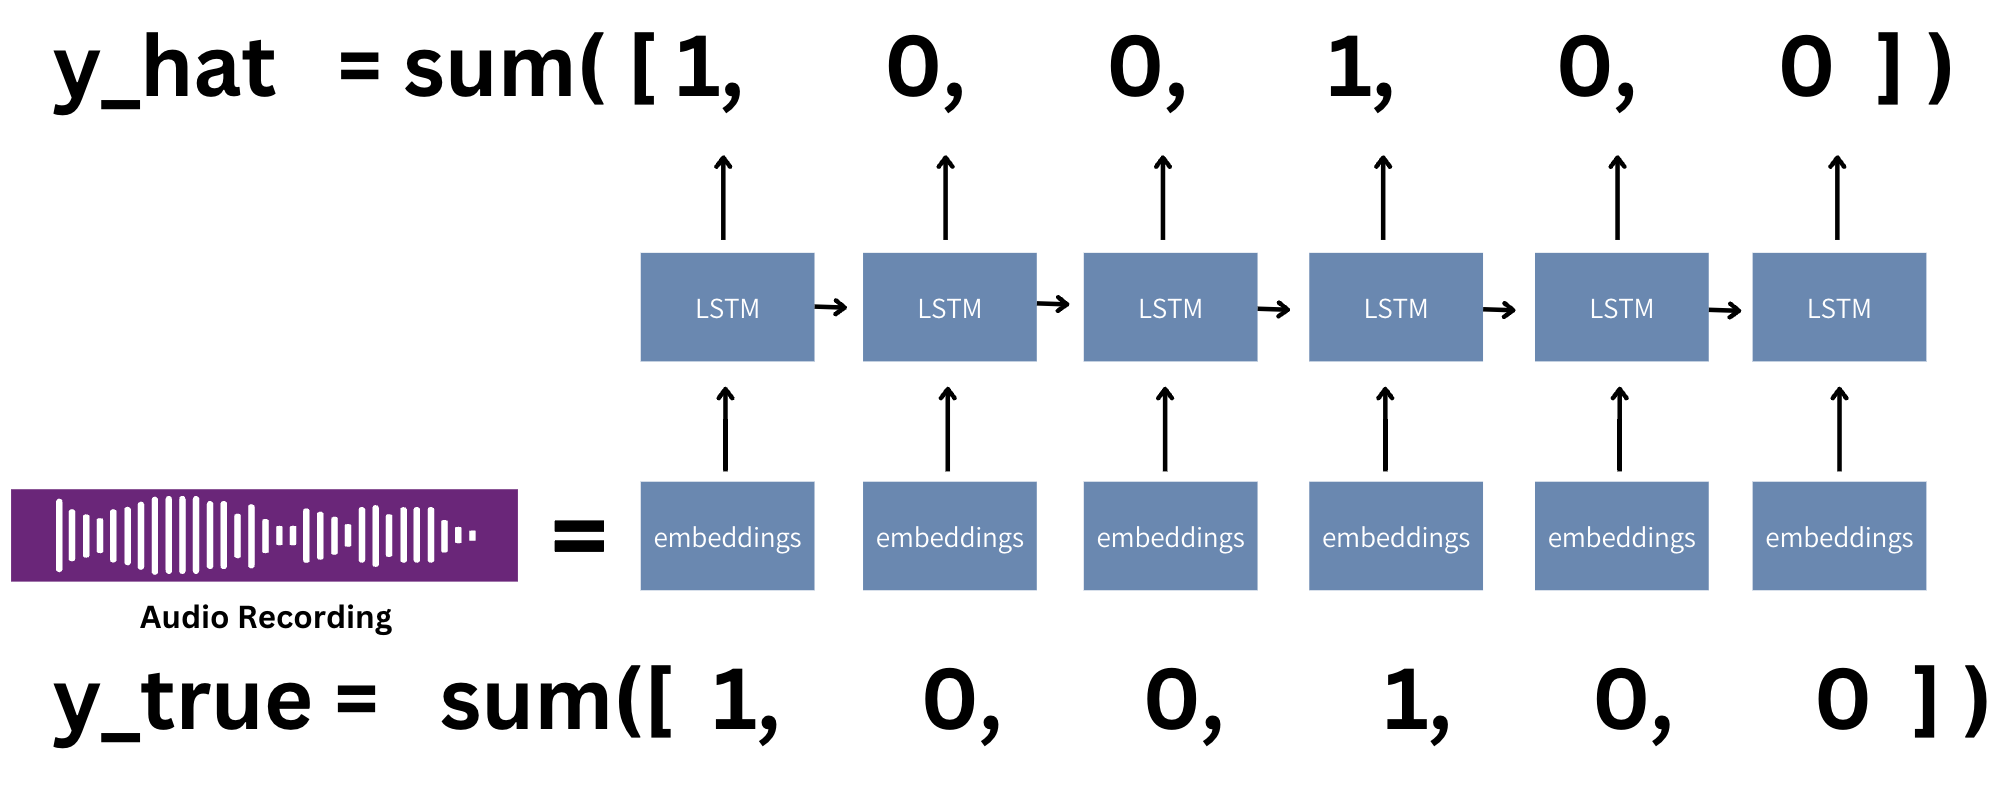
\includegraphics[scale=0.25]{RNNdata.png}
    \caption{This diagram shows the input to the model. The 1 represents the `switch'. This diagram shows the input and the output of an audio recording with 2 singers.}
    \label{fig:embeddings}
\end{figure}

Our LSTM model is designed to recognize the distinct vocal timbre and style of each singer through embedded vocal clips. By analyzing the audio embeddings, which encapsulate various features of the sound such as pitch, tone, and rhythm, the model becomes adept at identifying even subtle shifts in these parameters, indicative of a change in the singer. 

The core of our approach lies in how we tally the number of distinct singers. As the LSTM processes the audio data, it flags moments where the vocal characteristics significantly differ from the preceding segment. These moments are considered 'switches' in singers. After outputing the predicted switches, Our approach then aggregates these switches throughout the track, effectively counting the number of transitions from one singer to another.

\subsubsection{Model Implementation}
The model architecture consists of a Long Short-Term Memory (LSTM) Recurrent Neural Network implemented from scratch in PyTorch. 

$$L(y, \hat{y}) = -\frac{1}{N} \sum_{i=1}^{N} [y_i \cdot \log(\hat{y}_i) + (1 - y_i) \cdot \log(1 - \hat{y}_i)]$$

We optimized using Binary Cross Entropy loss (above) between the model output $ \hat{y}$ and the ground truth singer transition labels $y$. In this loss function, $y_i$ is the true label for the $i^{th}$ instance (which can be either 0 or 1), and $\hat{y}_i$ is the predicted probability that the $i^{th}$ instance belongs to the positive class (i.e., class 1). The sum is computed over all $N$ instances in the dataset. BCE suits the singer switch classification task as supports multi-class one-hot-encoded labels. Our model used Pytorch's implementation of Adam optimization algorithm to adjust learning rate and momentum of each epoch.

To validate our model's performance, we conducted extensive testing using a subset of the newly created `songs' not used in training. This allowed us to gauge the model's accuracy in real-world scenarios and make necessary adjustments to improve its efficacy. To evaluate accuracy, we used hamming loss. The outcome of this project holds promising implications for the future of automated vocal analysis in music production, offering a novel approach to understanding and dissecting complex audio recordings.

\section{Results}


\subsection{First Iteration: 2 Singers with No Randomization}
    Our earliest implementation of the RNN approach we used a dataset built of only $2$ singers, and each audio file split into $20$ chunks. 
    
    \subsubsection{Benchmarks: Clustering and Pyannote}
    The clustering algorithm achieved an impressive 75.68\% accuracy when we reduced the component to 1 and set the quantile at 0.5. In contrast, the pyannote model's accuracy was comparatively lower at 46.16\%. To determine these accuracy levels, we calculated the ratio of correctly classified audio clips to the total number of audio clips.

    \subsubsection{Sequential Chunk Processing with RNN}

    When we trained this model, we were happy to see it determining a function to accurately solve our task. The model's loss curve can be seen below (Fig. \ref{fig:rnn_loss_v1}).

    \begin{figure}[ht]
        \centering
        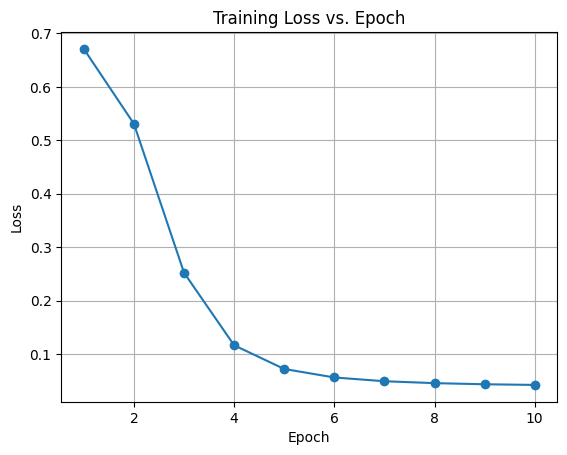
\includegraphics[scale=0.5]{RNN_Loss_v1.png}
        \caption{Loss curve during training from our initial implementation of the RNN.}
        \label{fig:rnn_loss_v1}
    \end{figure}
    
    However, this curve looks surprisingly smooth and an extremely low loss towards the end. Upon further investigation, we noticed that this model learned to predict a singer switch once at the beginning of the song, and once again halfway through the song. It ended up not learning how to identify singer changes, rather, a correlation of approximately when a change occurs.
    
    To address this critical issue, we modified the data slightly to reflect variations in a song's solo section lengths by adding noise to the lengths of our chunks. Instead of concatenating 5,000 millisecond (5 seconds) chunks of audio, we updated our method to concatenate between 2,000-5,000 milliseconds (2-5 seconds) of audio.

    Having made this adjustment, our loss curve looked nearly identical to before the change. By outputting the predictions from this new dataset, we found that the sparse labels of $2$ true switches among $20$ chunks caused the model to game the system and predict no switch for all chunks regardless of the input. \\

    \subsection{Second and Third Iteration: The Improved Model}
    Learning from these experiences, we decided to implement three changes: a) We varied the number of singers, now uniformly sampling from a range of 2 to 7, instead of just 2; b) We used 10 audio chunks, as opposed to 20; and c) During dataset generation, each singer's audio chunk was randomized to be between 2,000 and 5,000 milliseconds. These adjustments helped us tackle the issue of sparsity and made our data more representative of a context in which this model could be applied.


    \subsubsection{Benchmarks: Clustering and Pyannote}
    The clustering algorithm was configured with 3 components and a quantile of 0.25, resulting in an accuracy of 18\%. Meanwhile, the pyannote model underperformed, achieving a mere 7.5\% accuracy. 

    \subsubsection{Sequential Chunk Processing with RNN}
    After making these adjustments, the model's loss curve during training changed. The curve depicted by Fig. \ref{fig:rnn_loss_v2} shows the loss decreasing over time, which is a good sign that our model is learning from the training data. The consistent downward trend without any increase suggests that the model is converging well and not oscillating or overfitting during training. At the end of training, our model was able to accurately predict chunks with switches 64.50\% of the time. 
    
    \begin{figure}[ht]
        \centering
        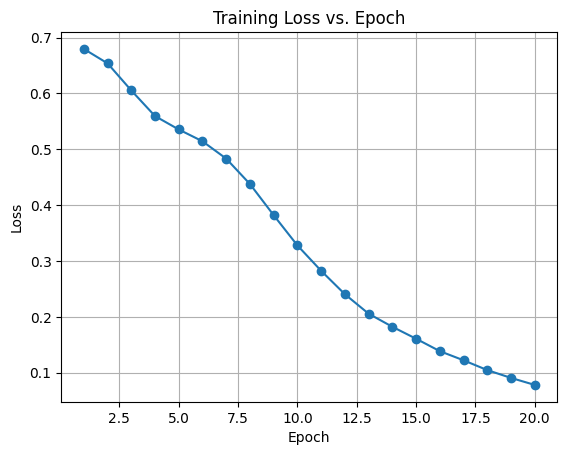
\includegraphics[scale=0.5]{RNN_Loss_v2.png}
        \caption{Loss curve during training from our final implementation of the RNN.}
        \label{fig:rnn_loss_v2}
    \end{figure}

    When comparing the predicted singer switches to actual counts, the magnitude of error (i.e. $|E|$) was within 2 90.00\% of the time, within 1 73.33\% of the time, and accurate 46.67\% of the time. 

    Additional results, as in the confusion matrices shown by Figures \ref{fig:rnn2_error}, \ref{fig:rnn2_conf_mat_pct}, and \ref{fig:rnn2_conf_mat} suggest that our model is generally able to correctly estimate how many voices are present in a recording. From the confusion matrices, the error rate appears to increase as the number of singers increase - this is something we plan to adjust for in future iterations of this model.

    \subsection{Summary of Results}
    Our RNN model exhibited commendable performance, achieving the highest accuracy of 45.6\% in datasets featuring a mix of 2-7 singers. The clustering algorithm excelled notably with configurations involving only 2 singers, while the pyannote model delivered average results under the same conditions. However, both models struggled in scenarios with a varied number of singers, particularly as the number increased. An encouraging sign is the steady learning trajectory observed in our RNN model, as evidenced by the consistently decreasing loss curve. This indicates potential for further improvement, and with additional fine-tuning, we are optimistic about enhancing the model's accuracy. 

\section{Discussion \& Future Improvements}
    The observed decrease in the clustering algorithm's accuracy when expanding the singer range from 2 to 2-7 highlights a potential limitation due to fixed parameter settings. The effectiveness of the algorithm seems contingent on the number of singers, suggesting a need for fine-tuning the PCA components and quantile levels accordingly. To enhance adaptability, we could explore the development of an algorithm or model capable of dynamically adjusting these parameters based on the number of singers being analyzed. Such a dynamic approach could significantly improve the algorithm's versatility and accuracy in diverse scenarios.

    It was unexpected to find that the pyannote speaker diarization model turned out to be the least accurate among all the methods we employed. This led to an important realization: models trained on spoken voice data differ significantly from those trained on singing data. Given that the pyannote model was developed for speaker data, its under-performance in our test, which featured recordings with varied pitch and tone, appears logical. To enhance the model's effectiveness for our purposes, fine-tuning it with our specific dataset is a viable option. However, this approach would demand considerable computational resources and necessitate new data processing techniques.

    A major insight from our work is the realization of the diverse methods available for data pre-processing and the substantial impact even slight modifications can have, as evidenced by the performance shifts in the RNN model. Going forward with the RNN model, our aim is to expand the dataset beyond the current count of 60 audio clips. We plan to increase the number of training epochs and dedicate more effort to refining the hyperparameters. Additionally, we are considering the integration of a bi-directional LSTM to enhance the model's capabilities. Furthermore, we are exploring the possibility of fine-tuning the SpeechBrain embedding model to specialize in processing singer data instead of speaker data, which could significantly alter our results.

\section{Resources Used}

    We utilized two pre-trained models for our project: the SpeechBrain EncoderClassifier and the Pyannote Speaker Diarization model. The code for implementing these models was sourced from Hugging Face. All of our data processing was implemented from scratch. Our RNN model was also developed from scratch using the PyTorch framework.

\newpage

\section*{References}
[1] C.-B. Jeon, H. Moon, K. Choi, B. S. Chon, and K. Lee, “Medleyvox: An evaluation dataset for multiple singing voices separation,” \textit{ICASSP 2023 - 2023 IEEE International Conference on Acoustics, Speech and Signal Processing (ICASSP)}, 2023. doi:10.1109/icassp49357.2023.10095425 

\vspace{0.25in}

[2] H. Bredin et al., “Pyannote.audio: Neural building blocks for speaker diarization,” ICASSP 2020 - 2020 IEEE International Conference on Acoustics, Speech and Signal Processing (ICASSP), 2020. doi:10.1109/icassp40776.2020.9052974

\vspace{0.25in}

[3] “Speechbrain/SPKREC-xvect-voxceleb · hugging face,” speechbrain/spkrec-xvect-voxceleb · Hugging Face, https://huggingface.co/speechbrain/spkrec-xvect-voxceleb (accessed Dec. 14, 2023). 

\vspace{0.25in}

[4] M. Ravanelli et al., “SpeechBrain: A General-Purpose Speech Toolkit.” ArXiv, 2021. Available: https://arxiv.org/pdf/2106.04624.pdf
‌

\clearpage
\section{Appendix}

\begin{figure}[ht]
    \centering
    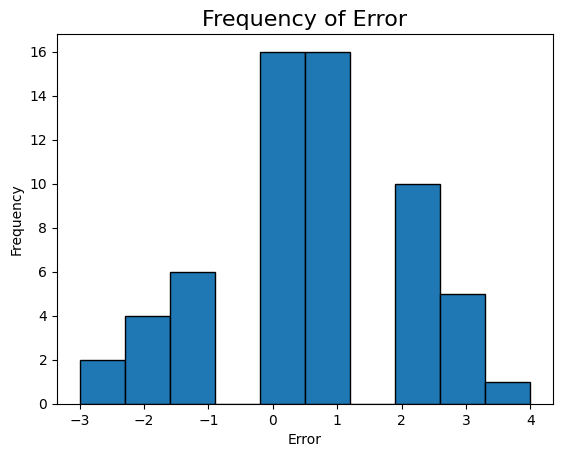
\includegraphics[scale=0.4]{RNN2_Error.png}
    \caption{A histogram of prediction error for our final RNN-based approach. Error is calculated as $y - \hat{y}$.}
    \label{fig:rnn2_error}
\end{figure}

\begin{figure}[ht]
    \centering
    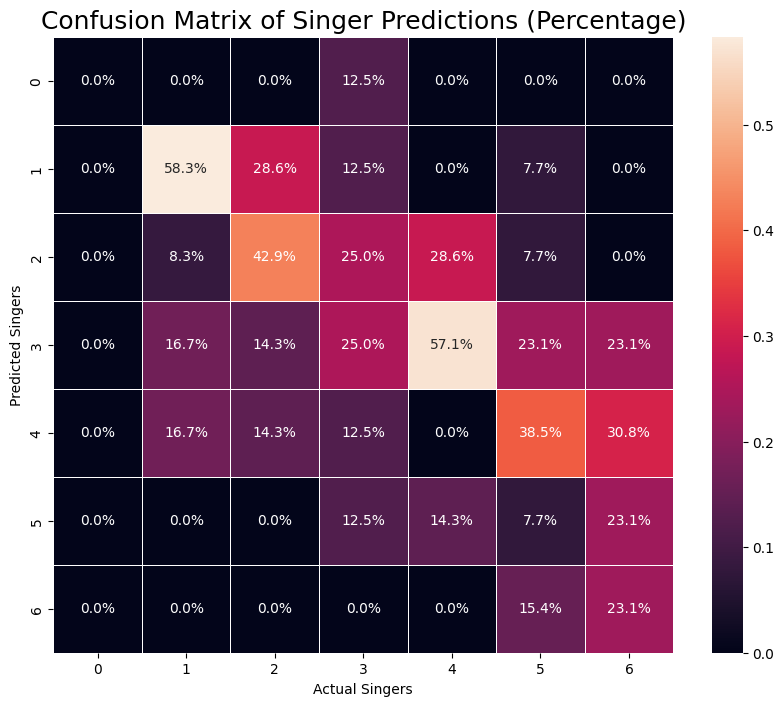
\includegraphics[scale=0.25]{RNN2_confusion_matrix_pct.png}
    \caption{The confusion matrix (in percentages) from our final RNN-based implementation. The strength along the diagonal is promising, showing that the model is able to estimate the number of switches quite well.}
    \label{fig:rnn2_conf_mat_pct}
\end{figure}

\begin{figure}[ht]
    \centering
    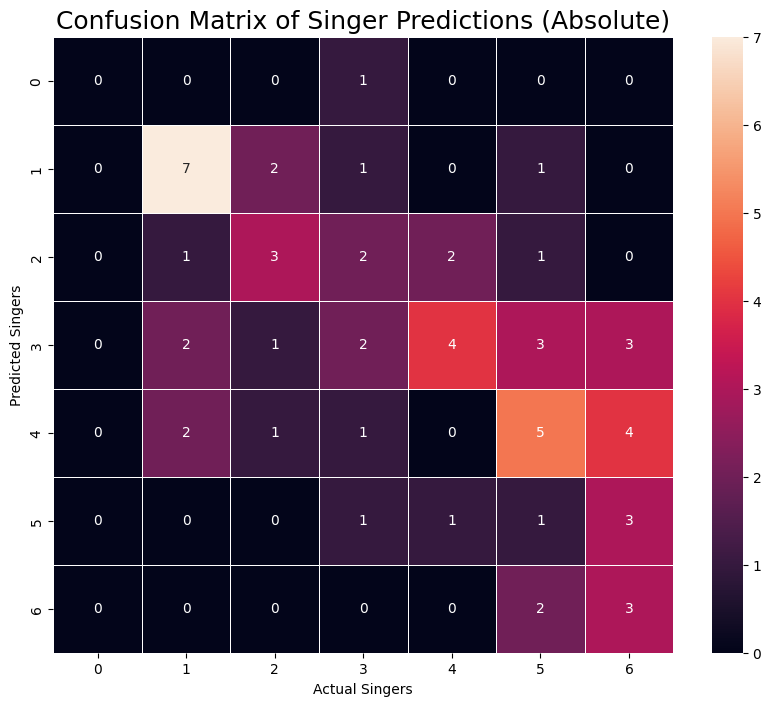
\includegraphics[scale=0.25]{RNN2_confusion_matrix.png}
    \caption{The confusion matrix (in absolute counts) from our final RNN-basd implementation. Note that the sample size in each column is quite small, so this may not be fully reflective of our model's capabilities and biases.}
    \label{fig:rnn2_conf_mat}
\end{figure}


\end{document}
